\section{Biography}

Haskell Brooks Curry\cite{enwiki:1192145129} (1900-1982) was an American mathematician and logician who made significant contributions to the field of mathematical logic and the theory of computation. He is best known for his work on combinatory logic, which is a formal system for expressing computation independent of the order of evaluation. Curry's work on combinatory logic laid the foundation for the development of functional programming languages, which are a class of programming languages that treat computation as the evaluation of mathematical functions and avoid changing-state and mutable data. The most famous functional programming language, Haskell, is named after him. In this paper, we will explore the life and work of Haskell Curry, and discuss his legacy in the field of computer science.

\begin{figure}[H]
    \centering
    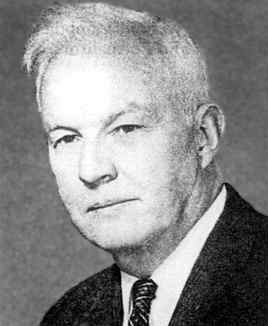
\includegraphics[width=0.5\textwidth]{figures/curry.jpg}
    \caption{Haskell Brooks Curry}
    \label{fig:curry}
\end{figure}




柯里16岁考入哈佛大学学医,不过中途转入数学系。本科毕业后在麻省理工学院电子工程系工作两年,后又返回哈佛学习物理,并取得硕士学位。在这期间,柯里因修读怀特海-罗素的《数学原理》课程开始对数理逻辑感兴趣,这促使他留在哈佛攻读数学专业博士学位。刚开始在他的导师George Birkoff指导下研究微分方程,但是柯里仍然放不下对数理逻辑的兴趣。1927年,柯里在普林斯顿大学获得讲师职务,期间发现了俄国学者Moses Schönfinkel在组合逻辑领域的研究,这激发起柯里极大的兴趣,并坚定了将此生投入到数理逻辑的研究当中。为此他远赴德国哥廷根,和熟悉Schönfinkel研究的两位学者Heinrich Behmann和Paul Burnays共同研究,在其导师、大名鼎鼎的希尔伯特指导下,以组合逻辑为内容完成论文获得了博士学位。

和大多数数理逻辑学家一样,柯里的研究中心也是数学基础问题,试图为数学找出一个安全的基础理论。1933年,柯里通过与John Rosser(也是一位值得提及的数理逻辑学家)通信得知了“Kleene-Rosser悖论”。这个理论由Kleene和Rosser共同研究,其结果分别证明了当时由阿隆佐·丘奇和柯里本人提出的几个形式系统的不完备性,而丘奇的系统,当时包括了λ-演算子系统,虽然整个系统不完备,但是这个子系统却是完备的。在这个证明完成之后,丘奇、Kleene和Rosser都放弃了对数学基础的研究,只有柯里坚持了下来,并声称“决不当悖论的逃兵”。
柯里对数学基础的全部希望都寄托在了“组合逻辑”上,这使他付出了毕生的精力。虽然组合逻辑的概念由Schönfinkel提出,但是大部分研究成果出自柯里,可以说柯里是组合逻辑的创建人之一。从现代角度来看,组合逻辑和λ-演算一同成为了函数式编程语言的理论基础,而后者的开创人正是阿隆佐·丘奇,不过丘奇的名声和$\lambda$-演算在很长一段时间内都盖过了柯里和组合逻辑。


Haskell Curry's mother was Anna Baright and his father was Samuel Silas Curry. Samuel was the president of the School of Expression in Boston and Anna was the Dean of the School. Haskell did not show particular interest in mathematics when at high school and when he graduated in 1916 he fully intended to study medicine. He entered Harvard College, the undergraduate school of Harvard University, and took a mathematics course in his first year of study as part of his studies towards a degree in medicine.

A major influence on the direction that his studies took was the entry of the United States into World War I in the spring of 1917. Curry wanted to serve his country, and decided that he would be more likely to see action if he had a mathematics training rather than if he continued the pre-medical course he was on. Anyhow he had enjoyed the mathematics course he had taken and had done very well in the course. He changed his major subject to mathematics and then enlisted in the Student Army Training Corps on 18 October 1918. The war, however, ended shortly after this (in November) and on 9 December 1918 Curry left the army. He continued on the mathematics course at Harvard, however, and graduated in 1920 with an A.B. degree.

Curry now decided that he would look for a career in electrical engineering and he took a job with the General Electric Company which allowed him to study electrical engineering part-time at the Massachusetts Institute of Technology. However he soon discovered that he had a different attitude to the others taking the courses, for he wanted to know why a result was correct when for everyone else it only mattered that it was correct. Realising that he was more suited to pure science than to applied science, he changed course to study physics in 1922. Also Harvard seemed a better place to study pure science so he returned there, having been appointed to a half-post as a research assistant of P W Bridgeman for the session 1922-23. Curry graduated with a Master's Degree in physics from Harvard in 1924 but by now he realised that the subject for him was not physics but it was mathematics. He began to undertake research for his doctorate in mathematics at Harvard.

Throughout this period of changing topics Curry had other things to keep him busy. His father had died in 1921 and Curry became a trustee of his father's estate. Of course the main part of this estate was the School of Expression in Boston and, three years after the death of Curry's mother in 1924, it became a legal corporation in 1927. Curry acted as treasurer to the Expression Company from the time it was formed, but it was sold in 1928.

If one imagines that from 1924 when Curry embarked on his doctorate in mathematics at Harvard he at last found the topic for him, then one would be mistaken. He was given a topic in the theory of differential equations by George Birkhoff but he began reading books on logic which seemed to him far more interesting that his research topic. He asked various faculty members at Harvard, and Norbert Wiener at MIT, if they thought he might change to undertake research in logic. They were quite unanimous, advising him against it. He was employed as a half-time instructor in mathematics by Harvard during the first semester of 1926-27 and it was around this time that he read the first volume of Whitehead and Russell's Principia Mathematica which had been published in 1910. This was fundamental in his development, for it was after reading this work that he had the idea to use combinators to analyse the complicated rules of substitution which characterise the first part of the text. He again approached various faculty members at Harvard, and Norbert Wiener at MIT, asking whether they thought that he might write his doctoral dissertation on logic. He now got a very different response from what he had received earlier. Wiener's reply was typical - avoid logic unless you have something to say, but now you certainly have something to say!

Curry now made his final change in direction and decided to give up his doctoral studies on differential equations and to write a doctoral dissertation on logic. Before beginning research on this new topic he decided to teach for a year and, with a strong recommendation from Birkhoff, was appointed as an instructor in mathematics at Princeton for session 1927-28. There he discussed his research plans with Veblen and, while looking at papers in Mathematische Annalen in the Princeton library, discovered a 1924 paper by M Schönfinkel Über die Bausteine der mathematischen Logik which used combinators in a similar way to his own ideas. Veblen assured Curry that this was a positive, rather than negative, discovery and, after Alexander had informed him that Schönfinkel was in a mental hospital and therefore not continuing his line of research, Curry sought advice on who would be the best Ph.D. supervisor. Veblen advised him that Bernays at Göttingen, in Germany, would be best. In order to improve his chances of financial support, Curry wrote up his ideas on combinators for publication and this became his first paper An analysis of logical substitution which appeared in the American Journal of Mathematics in 1929.

Before setting off for Göttingen, Curry married Mary Virginia Wheatley whom he had met at the School of Expression when she was a student there. They married on 3 July 1928 and travelled together to Germany. After almost exactly a year (on 24 July 1929) he was examined on his thesis entitled Grundlagen der kombinatorischen Logik. Formally he was supervised by Hilbert, but in fact it was Bernays who provided day to day support for his work. His dissertation was published in the American Journal of Mathematics in 1930.

Returning to the United States, Curry was appointed to State College, Pennsylvania (now Pennsylvania State University) in September 1929. Haskell and Virginia began their family at this time with Anne Wright Curry born on 27 July 1930 and Robert Wheatley Curry born on 6 July 1934. The Great Depression began in 1929 so it was fortunate that Curry obtained his position when he did. Certainly the years of the Great Depression would have been ones when a mathematical logician would hardly have been likely to obtain a post. Although he remained on the faculty at Pennsylvania State until he retired in 1966, he did spend time at other institutions, particularly at the University of Chicago, where he was a National Research Council Fellow during 1931-32, and the Institute for Advanced Study at Princeton during 1938-39. Some papers published during the early years of his research include The universal quantifier in combinatory logic (1931), Some additions to the theory of combinators (1932), Apparent variables from the standpoint of combinatory logic (1933), and Some properties of equality and implication in combinatory logic (1934).

The Association for Symbolic Logic was founded in 1936 with Curry as one of the founders. He was vice-president during 1936-37 and then president of the Association in 1938-40. His retiring presidential address The combinatory foundations of mathematical logic was published in the Journal of Symbolic Logic in 1942. After giving a very clear exposition of the fundamentals of combinatory logic, showing its close relationship to the λ-calculus developed by Church, Curry went on to describe his recent work. He had examined simplified methods of deriving the paradoxes (such as those of Richard and Russell) in systems of logic which are inconsistent, and had also developed a method of introducing into combinatory logic undefined notions of generality, such as quantification or formal implication, in such a way that a consistency theorem like that of Church and Rosser could still be derived.

As the 1940s began, Curry had reached the position of being one of the leading mathematical logicians in the world. He was asked to give an expository address to mathematicians to explain the fundamental concepts of formalism and to add new suggestions. The paper Some aspects of the problem of mathematical rigor published in the Bulletin of the American Mathematical Society in 1941 is the text of this address. He presented in his address: a critique of non-formal theories; the notion of a formal system (illustrated by Dickson's postulates for a group); the notion of a calculus; discussion of a metatheory; the definition of mathematics; and acceptability of a formal system, discussing criticisms from intuitionists and formalists. During the 1940s Curry also renewed his association with the School of Expression in Boston, which by this time had been renamed Curry College. He joined the Board of Trustees of the College in 1940 and remained on the Board for over a decade.

During World War II Curry undertook research in applied mathematics. He published The Heaviside operational calculus in 1943. In it he presented a very simple algebraic approach but was aware of its limitations writing:-
... this advantage, of course, implies a restriction on the scope of the treatment, because it is limited to the rational aspects such as arise from ordinary linear differential equations with constant coefficients. For the more general cases of partial differential equations, fractional operators, etc., the theory of integral transforms is doubtless unavoidable.
He worked at the Frankford Arsenal from May 1942 to January 1944, then at the Applied Physics Laboratories at Johns Hopkins University until March 1945. He then went to the Aberdeen Proving Ground, a military weapons testing site in Harford county northeastern Maryland. There he became involved with the ENIAC computer publishing A study of inverse interpolation on the ENIAC and A study of fourth order interpolation on the ENIAC both in 1946. He returned to Pennsylvania State University in September 1946 and tried to persuade the University authorities to acquire a computer, but he failed.

His major texts include Combinatory Logic (1958) (with Robert Feys), and Foundations of Mathematical Logic (1963). Curry began working on Combinatory Logic in 1950 when he was awarded a Fulbright Grant that enabled him to work with Robert Feys at Louvain. They continued collaborating on the book after Curry returned to the United States and completed the text in 1956. E J Cogan, reviewing the book, gives a nice description of combinatory logic:-
Combinatory logic is concerned with certain basic notions of the foundations of mathematics which are usually used in an intuitive and unanalysed way. Such notions include substitution, usually introduced by the use of variables, and classification of the entities of a system into types, which is usually provided for by rules which are auxiliary to, but not part of, the system. The part of combinatory logic which is concerned with questions of a fundamental nature which, like substitution, involve variables, is called the theory of combinators.
In Foundations of Mathematical Logic Curry develops the topic from an algebraic basis using Gentzen's methods. J Tucker writes:-
The most striking effect of this approach is that the finite positive operations of implication, conjunction and alternation are dealt with first, while negation and quantification are brought in later and in separate chapters. The meaning of each fundamental connective is not laid down at the beginning as it is in the classical approach, but is derived by inferential rules.
In 1966 he accepted the position of Professor of Logic, History of Logic, and Philosophy of Science at Amsterdam. He held this position for four years after which he returned to live in State College, Pennsylvania.

The authors of [3] make some nice comments about Curry and his wife:-
Everyone who knows the Currys is aware of how friendly and helpful they always are. Haskell has always done more for colleagues and students than be a source of important ideas. He has always been willing to listen to everyone who wanted to talk to him, to discuss their ideas, and to give whatever encouragement that he could. ... His office door has always been open. And this has undoubtedly been an important contribution to the enthusiasm of many of those of us working in combinatory logic. Also well known wherever the Currys have lived has been the hospitality they have shown. There are always many parties and other, less formal gatherings, and we conjecture that Virginia's cooking has also played a role in the growth of interest in combinatory logic.
